
\documentclass{article}[14pt]
\usepackage{multicol, enumerate, enumitem, hyperref, color, soul, setspace, parskip, fancyhdr, amssymb, amsthm, amsmath, bbm, latexsym, units, mathtools}
\everymath{\displaystyle}
\usepackage[headsep=0.5cm,headheight=0cm, left=1 in,right= 1 in,top= 1 in,bottom= 1 in]{geometry}
\pagestyle{fancy}
\lhead{}
\chead{Answer Key for Module\,6\,-\,Polynomial\,Functions Version B}
\rhead{}
\lfoot{Summer\,C\,2020}
\cfoot{}
\rfoot{}
\begin{document}
\textbf{This key should allow you to understand why you choose the option you did (beyond just getting a question right or wrong). \href{https://xronos.clas.ufl.edu/mac1105spring2020/courseDescriptionAndMisc/Exams/LearningFromResults}{More instructions on how to use this key can be found here}.}

\textbf{If you have a suggestion to make the keys better, \href{https://forms.gle/CZkbZmPbC9XALEE88}{please fill out the short survey here}.}

\textit{Note: This key is auto-generated and may contain issues and/or errors. The keys are reviewed after each exam to ensure grading is done accurately. If there are issues (like duplicate options), they are noted in the offline gradebook. The keys are a work-in-progress to give students as many resources to improve as possible.}

\rule{\textwidth}{0.4pt}

26. Construct the lowest-degree polynomial given the zeros below. Then, choose the intervals that contain the coefficients of the polynomial in the form $x^3+bx^2+cx+d$.
$$ 4 - 5i \text{ and } 4 $$ 
The solution is $ x^{3} -12 x^{2} +73 x -164 $ 

\begin{enumerate}[label=\Alph*.] 
\item $ b \in [-17, -8], c \in [72, 75], \text{ and } d \in [-165, -158] $ 

 * $x^{3} -12 x^{2} +73 x -164$, which is the correct option. 
\item $ b \in [0, 3], c \in [-7, 4], \text{ and } d \in [-27, -16] $ 

 $x^{3} + x^{2} +x -20$, which corresponds to multiplying out $(x + 5)(x -4)$. 
\item $ b \in [9, 17], c \in [72, 75], \text{ and } d \in [162, 169] $ 

 $x^{3} +12 x^{2} +73 x + 164$, which corresponds to multiplying out $(x-(4 - 5i))(x-(4 + 5i))(x + 4)$. 
\item $ b \in [0, 3], c \in [-9, -4], \text{ and } d \in [10, 22] $ 

 $x^{3} + x^{2} -8 x + 16$, which corresponds to multiplying out $(x -4)(x -4)$. 
\item $ \text{None of the above.} $ 

 This corresponds to making an unanticipated error or not understanding how to use nonreal complex numbers to create the lowest-degree polynomial. If you chose this and are not sure what you did wrong, please contact the coordinator for help. 
\end{enumerate} 
 
General Comments: Remember that the conjugate of $a+bi$ is $a-bi$. Since these zeros always come in pairs, we need to multiply out $(x-(4 - 5i))(x-(4 + 5i))(x-(4))$.

-----------------------------------------------

27. Describe the zero behavior of the zero $x = 9$ of the polynomial below.
$$ f(x) = -7(x - 3)^{10}(x + 3)^{8}(x - 9)^{5}(x + 9)^{2} $$ 

 
 The solution is  
 \begin{center} 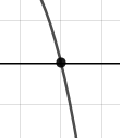
\includegraphics[width=0.3\textwidth]{../Figures/zeroBehaviorNegativeOddB.png} \end{center}\begin{tabular}{|c|c|} 
\hline 
 & \tabularnewline 
 \textbf{A.} 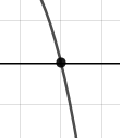
\includegraphics[width=0.3\textwidth]{../Figures/zeroBehaviorNegativeOddB.png} & \textbf{B.} 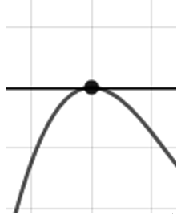
\includegraphics[width=0.3\textwidth]{../Figures/zeroBehaviorNegativeEvenB.png} \tabularnewline 
\hline 
 & \tabularnewline 
 \textbf{C.} 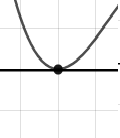
\includegraphics[width=0.3\textwidth]{../Figures/zeroBehaviorPositiveEvenB.png} & \textbf{D.} 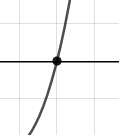
\includegraphics[width=0.3\textwidth]{../Figures/zeroBehaviorPositiveOddB.png} \tabularnewline 
\hline 
 E. None of the figures above. & \tabularnewline 
\hline 
 \end{tabular} 
 
\textbf{General Comments:} You will need to sketch the entire graph, then zoom in on the zero the question asks about.

-----------------------------------------------

28. Which of the following equations \textit{could} be of the graph presented below?
\begin{center} 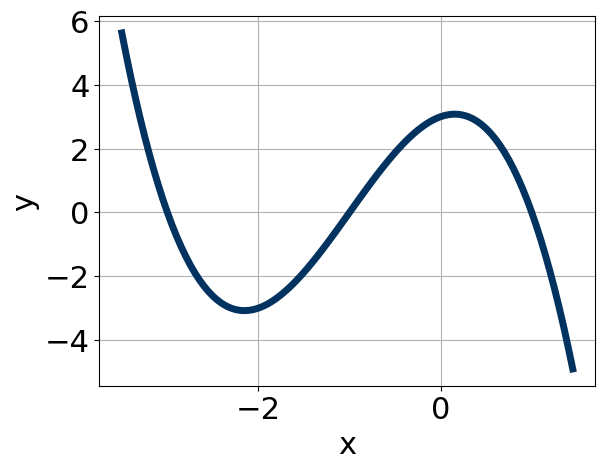
\includegraphics[width=0.3\textwidth]{../Figures/polyGraphToFunctionB.png} \end{center} 

The solution is $ -6(x - 1)^{6} (x + 3)^{7} (x + 1)^{7} $ 

\begin{enumerate}[label=\Alph*.] 
\item $ -6(x - 1)^{10} (x + 3)^{8} (x + 1)^{9} $ 

 The factor $(x + 3)$ should have an odd power. 
\item $ 19(x - 1)^{10} (x + 3)^{11} (x + 1)^{7} $ 

 This corresponds to the leading coefficient being the opposite value than it should be. 
\item $ -6(x - 1)^{6} (x + 3)^{7} (x + 1)^{7} $ 

 * This is the correct option. 
\item $ -2(x - 1)^{9} (x + 3)^{10} (x + 1)^{11} $ 

 The factor $1$ should have an even power and the factor $-3$ should have an odd power. 
\item $ 4(x - 1)^{10} (x + 3)^{9} (x + 1)^{6} $ 

 The factor $(x + 1)$ should have an odd power and the leading coefficient should be the opposite sign. 
\end{enumerate} 
 
General Comments: Draw the x-axis to determine which zeros are touching (and so have even multiplicity) or cross (and have odd multiplicity).

-----------------------------------------------

29. Describe the end behavior of the polynomial below.
$$ f(x) = -3(x - 7)^{5}(x + 7)^{10}(x + 4)^{2}(x - 4)^{4} $$ 

 
 The solution is  
 \begin{center} 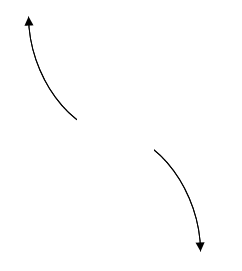
\includegraphics[width=0.3\textwidth]{../Figures/endBehaviorNegativeOddB.png} \end{center}\begin{tabular}{|c|c|} 
\hline 
 & \tabularnewline 
 \textbf{A.} 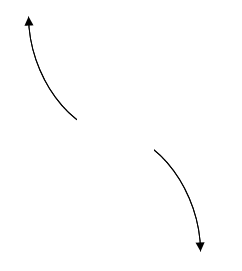
\includegraphics[width=0.3\textwidth]{../Figures/endBehaviorNegativeOddB.png} & \textbf{B.} 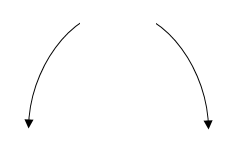
\includegraphics[width=0.3\textwidth]{../Figures/endBehaviorNegativeEvenB.png} \tabularnewline 
\hline 
 & \tabularnewline 
 \textbf{C.} 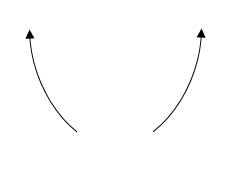
\includegraphics[width=0.3\textwidth]{../Figures/endBehaviorPositiveEvenB.png} & \textbf{D.} 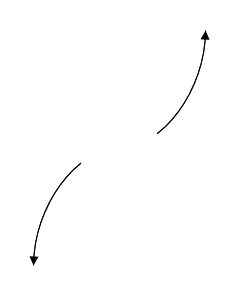
\includegraphics[width=0.3\textwidth]{../Figures/endBehaviorPositiveOddB.png} \tabularnewline 
\hline 
 E. None of the figures above. & \tabularnewline 
\hline 
 \end{tabular} 
 
\textbf{General Comments:} Remember that end behavior is determined by the leading coefficient AND whether the \textbf{sum} of the multiplicities is positive or negative.

-----------------------------------------------

30. Construct the lowest-degree polynomial given the zeros below. Then, choose the intervals that contain the coefficients of the polynomial in the form $ax^3+bx^2+cx+d$.
$$ \frac{1}{2}, \frac{6}{5}, \text{ and } \frac{5}{3} $$ 
The solution is $ 30x^{3} -101 x^{2} +103 x -30 $ 

\begin{enumerate}[label=\Alph*.] 
\item $ a \in [29, 35], b \in [-102, -98], c \in [102, 106], \text{ and } d \in [-36, -28] $ 

 * $30x^{3} -101 x^{2} +103 x -30$, which is the correct option. 
\item $ a \in [29, 35], b \in [100, 103], c \in [102, 106], \text{ and } d \in [25, 33] $ 

 $30x^{3} +101 x^{2} +103 x + 30$, which corresponds to multiplying out $(2x + 1)(5x + 6)(3x + 5)$. 
\item $ a \in [29, 35], b \in [-102, -98], c \in [102, 106], \text{ and } d \in [25, 33] $ 

 $30x^{3} -101 x^{2} +103 x + 30$, which corresponds to multiplying everything correctly except the constant term. 
\item $ a \in [29, 35], b \in [-82, -69], c \in [15, 19], \text{ and } d \in [25, 33] $ 

 $30x^{3} -71 x^{2} +17 x + 30$, which corresponds to multiplying out $(2x + 2)(5x -5)(3x -3)$. 
\item $ a \in [29, 35], b \in [-3, 2], c \in [-71, -61], \text{ and } d \in [-36, -28] $ 

 $30x^{3} + x^{2} -67 x -30$, which corresponds to multiplying out $(2x + 2)(5x + 5)(3x -3)$. 
\end{enumerate} 
 
General Comments: To construct the lowest-degree polynomial, you want to multiply out $(2x -1)(5x -6)(3x -5)$

-----------------------------------------------


\end{document}

